%!TEX root =  ../main.tex


\mychapters{Identities}{identities}{\chapdir/pics/PIA05380} 

Trigonometry is like the Hydra of ancient legends: you cut off one head, only to have
three more erupt out.  The interrelated nature of the circle and the reference triangle
mean there are an infinite number of ways to express the same function, via
trigonometric functions.


\newpage
\chapterminitoc


%									10 - 1
\newpage
\invisiblesection{Simple Trigonometric Equations}
\subsection{Lab}
word doc
%!TEX root =  ../main.tex

\subsection{Sine Slices}
Trigonometric equations are unlike linear equations, in that they have infinitely many
answers.  We typically answer them over a domain like $\theta \in \left[0,\tau\right]$ or
$\theta \in \left[\-\frac{\tau}{2},\frac{\tau}{2}\right]$.  Let us begin by finding a way to
express the infinite solution set.

\marginfig[-0.5in]{\chapdir/pics/Sin_unit_circle.png}{The height achieved by turning 
angle $\alpha$ will reoccur in one other place\label{fig:sinecircle}.}
Suppose we want to find all the answers to a simple equation
\begin{equation}\label{eq:sinx12}
\sin(x) = \frac{1}{2}
\end{equation}
With the Unit Circle memorized, we can easily recall that this happens at 
$\frac{\tau}{12}$.  However, we know that sine is $y$ on the Unit Circle, and so it
will come up again and again.  As Fig.~\ref{fig:sinecircle} shows, the height will
reoccur at $\frac{\tau}{2}-\theta$.  We also can add or subtract as many full-rotations
(i.e. $\tau$) as we like, and still get the same height.  This means that the full
solutions set for Eq.~\ref{eq:sinx12} is
$$
x  = \begin{cases} \frac{\tau}{12} & \pm k\tau\\
\frac{11\tau}{12} & \pm k\tau \end{cases} 
$$
where $k \in \mathbb{W}$.  Or the more general solution for $\sin\theta=x$:
\begin{equation}
\theta  = \begin{cases} \sin^{-1}(x) & \pm k\tau\\
\frac{\tau}{2} - \sin^{-1}(x) & \pm k\tau \end{cases} 
\end{equation}
Notice that only if $\sin^{-1}(x)$ is known can these be resolved without a
calculator.

\subsection{Cosine Cuts}
\marginfig[0in]{\chapdir/pics/Cos_unit_circle.png}{The horizontal displacement 
achieved by turning  angle $\alpha$ will reoccur in one other place\label{fig:cosinecircle}.}
Substitution can help prevent confusion when there are confusing extras like (e.g. $\theta-17$) inside
There can be quadratics etc, which substitution make clearer.  In general, if you find
yourself distracted or daunted by a bit of notation, remove it from sight for a moment and
solve the easier part, before bringing back the difficulty.

Consider the broad question, asked without domain restrictions
\begin{equation}
\cos(x) = -\frac{1}{2}
\end{equation}
This should be read in our minds in a clear verbal language as, ``What angles $x$ can be
turned from standard position the produce horizontal displacements of 0.5 to the left?''
Hopefully, this restatement allows us to visualize that both a third and fourth
quadrant angle exist that have the same $x$ value.  Because these angle can be reached by
turning the same amount clockwise or counter-clockwise, we can write our answer
succinctly as 
$$
x= \pm\frac{\tau}{3} \pm k\tau
$$
Universally, the solution to $\cos\theta = x$ is
\begin{equation}
\theta = \pm\cos^{-1}(x) \pm k\tau
\end{equation}

Now, if we are solving an equation with a strange term, we are still able to see the
answers clearly through substitution.  For example, 
$$
2 \cos (\theta - 17^\circ) = 1
$$
invites us to divide by two, but what then?  It is clarifying to substitute in the expression
\begin{equation}
u = \theta - 17
\end{equation}
A perfectly valid move, provided with undo it before the end.  If $\cos u = \frac{1}{2}$, our
answers in degrees are $u = \pm60^\circ \pm k\tau$, but we have answered in the wrong
variable.  ``Unsubstituting'', we get
\begin{equation}
\theta - 17^\circ = \begin{cases} 60^\circ & \pm k\tau \\ -60^\circ & \pm k\tau \end{cases}
\end{equation}
Perhaps you have not experienced manipulated equations with cases in them.  It is no
surprise that we simple add 17 to both sides, only on the right there are two places to do so.
Final answers:
$$
\theta = \begin{cases} 77^\circ & \pm k\tau \\ -43^\circ & \pm k\tau \end{cases}
$$

\subsection{Tangent Tilts}
Lastly, tangent can be the easiest to deal with, because it's period is less than one
full rotation.  Thinking back to the unit circle, slopes are the same in the first and third
quadrant, and again in the second and fourth.  This is because any line passing through
the origin is identical if rotated $\frac{\tau}{2}$.  

\begin{example}
	\exProblem
Factor and solve $\tan^2\theta - 2\tan\theta - 3 = 0$ for all it solutions.

	\exSolution
If it is not obvious that this is a quadratic in tangent, we can substitute $u = \tan\theta$ to
get $u^2 - 2u - 3 = 0$, and un-substitute later.  This factors easily into $(u-3)(u+1)=0$, which
means $u = \{3, -1\}$.  Asking when tangent equals -1 is the same as asking, ``For what
angles is the slope -1?''  These are all the angles beginning with a $\frac{\tau}{8}$ reference
angle in the second quadrant, and every half-rotation after that, i.e. $\frac{3\tau}{8}+\frac{\tau}{2}k$.
The angle of a slope of 3 is not a rational number, but the TI-8* says it is approximately
1.25, so we can write $1.25 + \frac{\tau}{2}k$.
\end{example}


The period can be off, so consider making a general solution and using it to generate answers

\newpage
\subsection{Exercises}
done in Kuta


%									10 - 2
\newpage
\section{Co-function, Pythagorean, Even/Odd}
\subsection{Problems}
In Word.
\newpage
%!TEX root =  ../main.tex

\subsection{Reference Triangle Within}
\subsection{Reference Triangles Without}
\subsection{Full Geometry}
\subsection{Algebra Ratios}
\subsection{Time Savers}
\subsection{Conjugates}

\newpage
\subsection{Exercises}
in Kuta


%									10 - 3
\newpage
\invisiblesection{Sum and Difference Identities}
\marginlessinput{\chapdir/1003p}
\newpage
\subsection{Cosine Sum and Difference}
insert diagram from wikipedia.

We believe the most elegant proof of the Cosine Sum of Angles formula is the
rectangle above, which you constructed in the lab.  Only slightly less aesthetically appealing
(unless you are afraid of long algebra expression, in which case you will find it drastically
less appealing) is a proof using the distance formula.  Suppose we have two angles inside
a unit circle, $\alpha$ and $\beta$.  We might stack them on top of each other, beginning at
standard position, and putting $\alpha$ in first.  Using the tools of analytic geometry at your
disposal, it should be easy to compute that a turn of $\alpha$ takes us to the point
$(\cos\alpha, \sin\alpha)$ and that a turn of $\alpha+\beta$ takes us to the point 
$(\cos(\alpha+\beta), \sin(\alpha+\beta)$.  A turn of 0 leaves us at (1,0).

insert diagram

While it is obvious that $\cos(\alpha+\beta) \ne \cos\alpha + \cos\beta$, it is by no means clear
what it \emph{does} equal from the diagram.  The clever trick is to then proceed from 0 by a turn
of $-\beta$.  Using the definition of sine's and cosine's evenness or oddness, we see that this turn
takes us to $(\cos\beta, -\sin\beta)$.  Now we have two congruent triangles, both with two sides
of length 1, and central angles of $\alpha+\beta$.  Therefore, their sides opposite that angle 
must be congruent.  We can solve two distance formulae, equal to each other.

insert final diagram

\begin{align*}
\sqrt{(\cos(\alpha+\beta)-1)^2 + (\sin(\alpha+\beta) - 0)^2} &= &\sqrt{(\cos\alpha-\cos\beta)^2 + (\sin\alpha - -\sin\beta)^2}\\
(\cos(\alpha+\beta)-1)^2 + \sin^2(\alpha+\beta) &= &(\cos\alpha-\cos\beta)^2 + (\sin\alpha - -\sin\beta)^2\\
\cos^2(\alpha+\beta) - 2\cos(\alpha+\beta) + 1 + \sin^2(\alpha+\beta) &= &\cos^2\alpha - 2\cos\alpha\cos\beta + \cos^2\beta + \sin^2\alpha + 2\sin\alpha\sin\beta + \sin^2\beta\\
\cos^2(\alpha+\beta) + \sin^2(\alpha+\beta) + 1 - 2\cos(\alpha+\beta) &= &\cos^2\alpha + \sin^2\alpha
+ \cos^2\beta + \sin^2\beta - 2\cos\alpha\cos\beta + 2\sin\alpha\sin\beta\\
1 + 1 - 2\cos(\alpha+\beta) &= &1 + 1 - 2\cos\alpha\cos\beta + 2\sin\alpha\sin\beta\\
\cos(\alpha+\beta) &=& \cos\alpha\cos\beta - \sin\alpha\sin\beta
\end{align*}

To find the Difference formula, we  plug in a $-\beta$ where we had a $\beta$ and simplify:

\begin{align*}
\cos\left(\alpha + (-\beta)\right) &=& \cos\alpha\cos(-\beta) - \sin\alpha\sin(-\beta)\\
\cos(\alpha - \beta) &=& \cos\alpha\cos\beta + \sin\alpha\sin\beta
\end{align*}

It is often convenient to write these two equations simultaneously, using the plus-or-minus
symbol on the left, and the minus-or-plus symbol on the right:

\begin{equation}
\cos(\alpha\pm\beta) = \cos\alpha\cos\beta \mp \sin\alpha\sin\beta
\end{equation}

\subsection{Sine Sum and Difference}
Because sine is the co-function cosine, we can continue to use algebra manipulation to make
the Sine Sum of Angles formula:

\begin{align*}
\sin(\alpha+\beta) &=& \cos\left(\frac{\tau}{4} - (\alpha + \beta)\right)\\
&=& \cos\left(\left(\frac{\tau}{4} - \alpha\right) - \beta\right)\\
&=& \cos\left(\frac{\tau}{4} - \alpha\right)\cos\beta + \sin\left(\frac{\tau}{4} - \alpha\right)\sin\beta\\
&=& \sin\alpha\cos\beta + \cos\alpha\sin\beta
\end{align*}

As before, we can substitute in a negative angle and get the Difference formula, but
that is left as an exercise for the reader.

\begin{equation}
\sin(\alpha \pm \beta) = \sin\alpha\cos\beta \pm \cos\alpha\sin\beta
\end{equation}

\subsection{Tangent Sum and Difference}

\begin{equation}
\tan(\alpha \pm \beta) = \frac{\tan\alpha \pm \tan\beta}{1 \mp \tan\alpha\tan\beta}
\end{equation}

\newpage
\subsection{Exercises}
in Kuta


%									10 - 4
%\newpage
\invisiblesection{Double Angles}
\subsection{Problems}
\noindent\makebox[\textwidth]{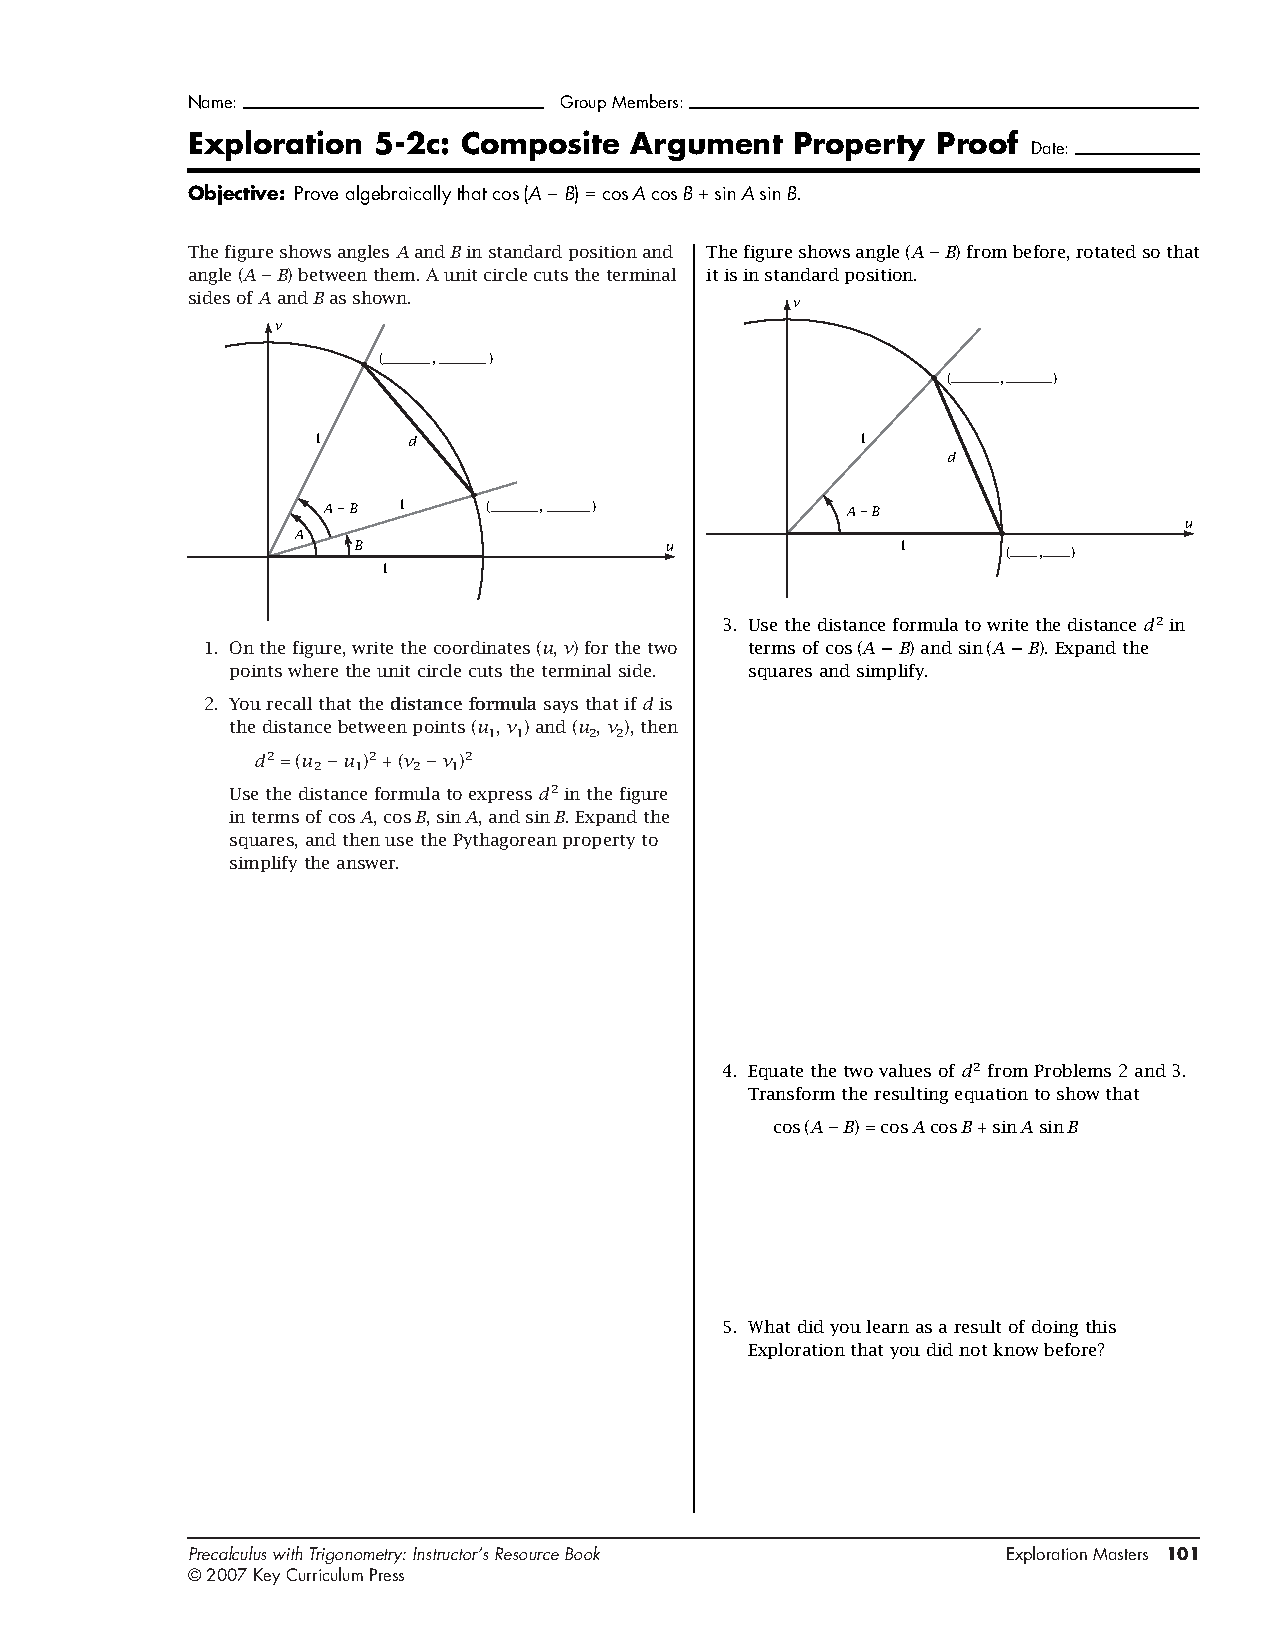
\includegraphics[width=\paperwidth]{\chapdir/1004p.pdf}}
\subsection{Double Sine and Tangent}
It might not seem worth it to memorize the double-angle formulas, since we can re-derive them
at will from the Sum of Angles formulae

\begin{equation}
\sin (\theta + \theta) = \sin\theta\cos\theta + \cos\theta\sin\theta\\
= 2\sin\theta\cos\theta
\end{equation}

As you can see, however, it is certainly a commonly encountered expression --- $\sin\theta\cos\theta$
--- and worth knowing that such can be transformed into $\frac{1}{2}\sin2\theta$.

\begin{equation}
\tan{\theta + \theta} = \frac{\tan\theta + \tan\theta}{1 - \tan\theta\tan\theta}\\
= \frac{2\tan\theta}{1 - \tan^2\theta}
\end{equation}

\subsection{Double Cosine}
But the cosine double angle formula is special:
\begin{equation}
\cos(\theta+\theta) = \cos\theta\cos\theta - \sin\theta\sin\theta\\
=\cos^2\theta - \sin^2\theta
\end{equation}

Because it involves $\cos^2\theta$ and $\sin^2\theta$, you should be reminded of the 
first Pythagorean Trigonometric Identity.  What happens is we substitute in the fact that
$\cos^2\theta = 1 - \sin^2\theta$?

\begin{equation}
\cos2\theta = (1 - \sin^2\theta) - \sin^2\theta\\
=1 - 2\sin^2\theta
\end{equation}

We might also have substituted the facts that $\sin^2\theta = 1 - \cos^2\theta$:

\begin{equation}
\cos2\theta = \cos^2\theta - (1 - \cos^2\theta)\\
=2\cos^2\theta - 1
\end{equation}

Apparently, there are three forms of the Cosine Double Angle Formula!  Because one involves
only sine, and one involves only cosine, these definitions are more or less useful in different
situations.  Careful deployment of the right one can save a lot of time.

\subsection{Half and Power}
Through basic manipulation, we can isolate either the sine-squared or the cosine-squared
from the previous two equations.

\begin{equation}
\cos^2\theta = \frac{1 + \cos2\theta}{2}
\end{equation}

\begin{equation}
\sin^2\theta = \frac{1 - \cos2\theta}{2}
\end{equation}

These are called the Power Reduction formulae, and while they ruin the angle, they are very
useful in calculus, especially in integrals.

Furthermore, we can see that the angle inside is twice the angle outside.  To help illustrate this, let
us substitute $u = 2\theta$:

\begin{align*}
\sin^2\left(\frac{u}{2}\right) & = & \frac{1 + \cos u}{2} \\
\sin\frac{u}{2} &=& \pm \sqrt{\frac{1 + \cos u}{2}} \\
& & \\
\cos^2\left(\frac{u}{2}\right) & = & \frac{1 - \cos u}{2} \\
\cos\frac{u}{2} & = & \pm \sqrt{\frac{1 - \cos u }{2}}
\end{align*}

Notice here that the plus-or-minus sign does not indicate what it normally does, that there are
two answers.  Instead, it means we must decide the sign of our answer.  This is an exercise
in the problem set.

\newpage
\subsection{Exercises}
done in Kuta


%									10 - 5
\newpage
\section{Proofs}
\subsection{Problems}
to be done in word
\newpage
\subsection{Summary of Trigonometric Derivatives}
\begin{equation}
\frac{d}{dx}\sin{x} = \cos{x}
\end{equation}
\begin{equation}
\frac{d}{dx}\cos{x} = -\sin{x}
\end{equation}
\begin{equation}
\frac{d}{dx}\tan{x} = \sec^2{x}
\end{equation}
\begin{equation}
\frac{d}{dx}\sec{x} = \sec{x}\tan{x}
\end{equation}
\begin{equation}
\frac{d}{dx}\sin^{-1}{x} = \frac{1}{\sqrt{1 - x^2}}
\end{equation}
\begin{equation}
\frac{d}{dx}\cos^{-1}{x} = -\frac{1}{\sqrt{1 - x^2}}
\end{equation}
\begin{equation}
\frac{d}{dx}\tan^{-1}{x} = \frac{1}{1 + x^2}
\end{equation}

\subsection{Summary of Trigonometric Integrals}
\begin{equation}
\int\sin{x}dx = -\cos{x} + C
\end{equation}
\begin{equation}
\int\cos{x}dx = \sin{x} + C
\end{equation}
\begin{equation}
\int\tan{x}dx = \ln{|\sec{x}|} + C
\end{equation}

\subsection{Summary of Trigonometric Identities}
\textbf{Even}: cosine, secant
\textbf{Odd}: sine, tangent, cosecant, cotangent
(Even functions exhibit the behavior $f(x) = f(-x)$.  Odd functions, that $f(-x)=-f(x)$.)

\subsubsection{Cofunctions}: sine and cosine, tangent and cotangent, secant and cosecant
(A cofunction is one that is the same as the other, only $90^\circ$ apart.  That is, 
$f(\frac{\tau}{4}-x) = g(x)$ and $g(\frac{\tau}{4}-x) = f(x)$.)

\subsubsection{Pythagorean Identities}
$\sin^2x + \cos^2x = 1$\\
$\tan^2x + 1 = \sec^2x$\\
$(1 + \cot^2x = \csc^2x$)

\subsubsection{Sum and Difference Identities}
$\sin(\alpha\pm\beta) = \sin\alpha\cos\beta \pm \cos\alpha\sin\beta$\\
$\cos(\alpha\pm\beta) = \cos\alpha\cos\beta \mp \sin\alpha\sin\beta$\\
$\tan(\alpha\pm\beta) = \frac{\tan\alpha\pm\tan\beta}{1\mp\tan\alpha\tan\beta}$

\subsubsection{Double Angle Formulae}
$\sin2u = 2\sin u \cos u$\\
$\cos2u = \cos^2u - \sin^2u = 2\cos^2u - 1 = 1 - 2\sin^2u$\\
$\tan2u = \frac{2\tan u}{1 - \tan^2u}$\\

\subsubsection{Half Angle Formulae}
$\sin\frac{u}{2} = \pm\sqrt{\frac{1-\cos u}{2}}$\\
$\cos\frac{u}{2} = \pm\sqrt{\frac{1+\cos u}{2}}$\\
$\tan\frac{u}{2} = \frac{1-\cos u}{\sin u} = \frac{\sin u}{1+\cos u}$\\


\subsubsection{Power Reduction Formulae}
$\sin^2\theta = \frac{1}{2}(1 - \cos\theta)$\\
$\cos^2\theta  = \frac{1}{2}(1 + \sin\theta)$

\subsection{Techniques for Proofs}
1. use only sine and cosine
2. multiply by the conjugate
3. always fix the angles first
4. substitute 

\newpage
\subsection{Exercises}
Prove that the area of a circle is pi r squared
\index{area!of a circle as an integral}
Prove that the area of an ellipse with radii a, b is abpi
\index{area!of an ellipse as an integral}
to be done in word


\newpage
\section{Review}
\subsection{Chapter Review}
\subsection{Chapter Test}